\documentclass[12pt]{article}\usepackage[margin=1in]{geometry}\usepackage{amsmath,amssymb,amsthm,graphicx,natbib,microtype}\newtheorem{theorem}{Theorem}\newtheorem{corollary}[theorem]{Corollary}
\title{Direct-Margin Scale Recurrence\\\large A Sharp Weyl Law and a Five-Scale Scalar-Alignment Barrier}\author{Prime Dynamics Theory Program}\date{July 2026}
\begin{document}\maketitle
\begin{abstract}
For a threshold $\tau$, define the direct support margin
$m_\tau(K)=s_4(K)-\tau s_1(K)$.  If, after unitary alignment and a scalar
scale $c\geq0$, the operator error is at most $\varepsilon$, then
\[
m_\tau(K')\geq c\,m_\tau(K)-(1+\tau)\varepsilon.
\]
The coefficients are sharp.  We also compute the optimal scalar Chebyshev
fit of finite singular profiles.  On 96 phase-matched archived pairs, only
26 endpoint fits and 6 four-mode fits retain a positive one-step lower; none
of 24 endpoint chains remains positive through all five scales.  Thus the
direct recurrence is rigorous, but the simplest scalar-alignment mechanism
is a poor finite route compared with RH-125.
\end{abstract}
\section{Sharp recurrence}
\begin{theorem}[Direct support-margin recurrence]\label{thm:margin}
Suppose $\|K'-cUKV\|\leq\varepsilon$ for unitaries $U,V$ and $c\geq0$.
Then for every $\tau\geq0$,
\[
m_\tau(K')\geq c\,m_\tau(K)-(1+\tau)\varepsilon.
\]
\end{theorem}
\begin{proof}
Weyl--Mirsky perturbation gives
$s_4(K')\geq cs_4(K)-\varepsilon$ and
$s_1(K')\leq cs_1(K)+\varepsilon$ \citep{HornJohnson1991}.  Subtraction
proves the result.
\end{proof}
The bound is sharp: take a diagonal operator with separated singular values
and perturb its leading entry upward by $\varepsilon$ and its fourth entry
downward by $\varepsilon$.

\begin{corollary}[Iteration]
If $m_{n+1}\geq c_nm_n-(1+\tau)\varepsilon_n$, then
\[
m_N\geq\Bigl(\prod_{j<N}c_j\Bigr)m_0-(1+\tau)
\sum_{k<N}\varepsilon_k\prod_{j=k+1}^{N-1}c_j.
\]
\end{corollary}

\section{Optimal scalar profile fit}
For positive profiles $s,t$, minimize
$\varepsilon(c)=\max_j|t_j-cs_j|$ over $c\geq0$.  Feasibility at radius
$\varepsilon$ is exactly the interval intersection
\[
\max_j\frac{t_j-\varepsilon}{s_j}\leq c\leq
\min_j\frac{t_j+\varepsilon}{s_j},\qquad c\geq0.
\]
This gives a monotone bisection with a certified minimax residual.  We use
both the endpoint profile $(s_1,s_4)$, which contains exactly the margin
information, and the stronger four-mode profile.

\section{Five-scale barrier}
The RH-121 archive supplies 96 adjacent pairs.  Every computed recurrence
lower is dominated by the target margin.  There are zero dominance failures.
Yet only 26 endpoint fits retain a
positive lower, and only 6 full-profile fits do.  Iterating the endpoint
recurrence along 24 side--threshold--phase chains leaves zero positive
terminal margins; the terminal range is approximately
$[-1.40\times10^{-2},-8.45\times10^{-11}]$.
\begin{figure}[h]\centering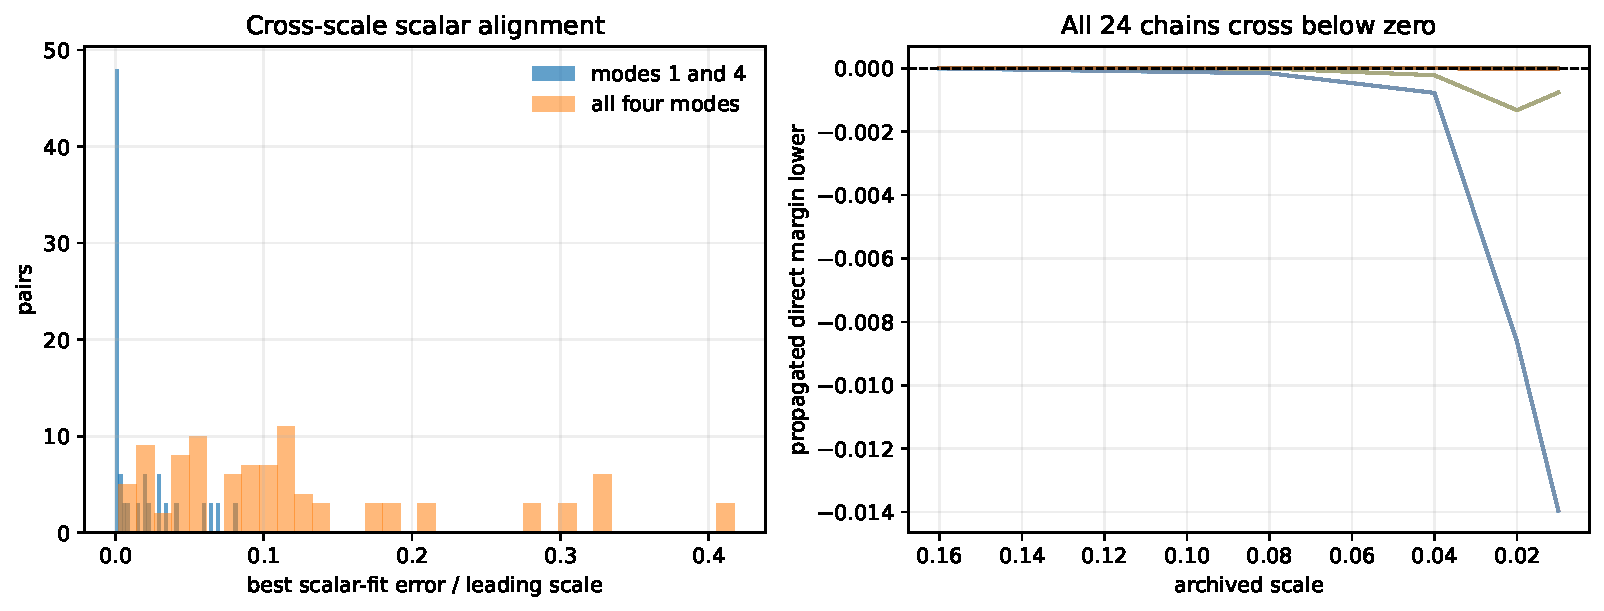
\includegraphics[width=\textwidth]{figures/direct_margin_scale_recurrence.pdf}\caption{Best scalar-profile errors and propagated direct margins.}\end{figure}

This is a finite negative result about scalar alignment, not a proof that
every direct physical recurrence is impossible.  An operator-valued source
law could still succeed.  The directional route remains primary, and RH-127
adds the outward guards it needs.  No uniform Stage A, Hilbert--Polya,
zeta-zero, or Riemann Hypothesis claim is made.
\bibliographystyle{plainnat}\bibliography{references}\end{document}
